\paragraph{二维支持集。}
\label{app:support_2d}
二维支持集包含来自11个数据集的259,767条源记录，覆盖医学论文图像、放射影像、病理图像及相关文本与标签。图~\ref{fig:support_composition}展示来源组成，表~\ref{tab:support_links}提供各数据集的官方资源链接。

\paragraph{三维支持集。}
\label{app:support_3d}
三维支持集包含来自5个数据集的215,657条源记录，其中包括209,329条问答与6,328条报告，覆盖解剖识别、定位、异常表征及报告生成。问答对应4,228个唯一视频，每个视频包含64帧有序切片。图~\ref{fig:support_composition}展示来源组成，表~\ref{tab:support_links}提供各数据集的官方资源链接。

\begin{figure}[!htb]
\centering
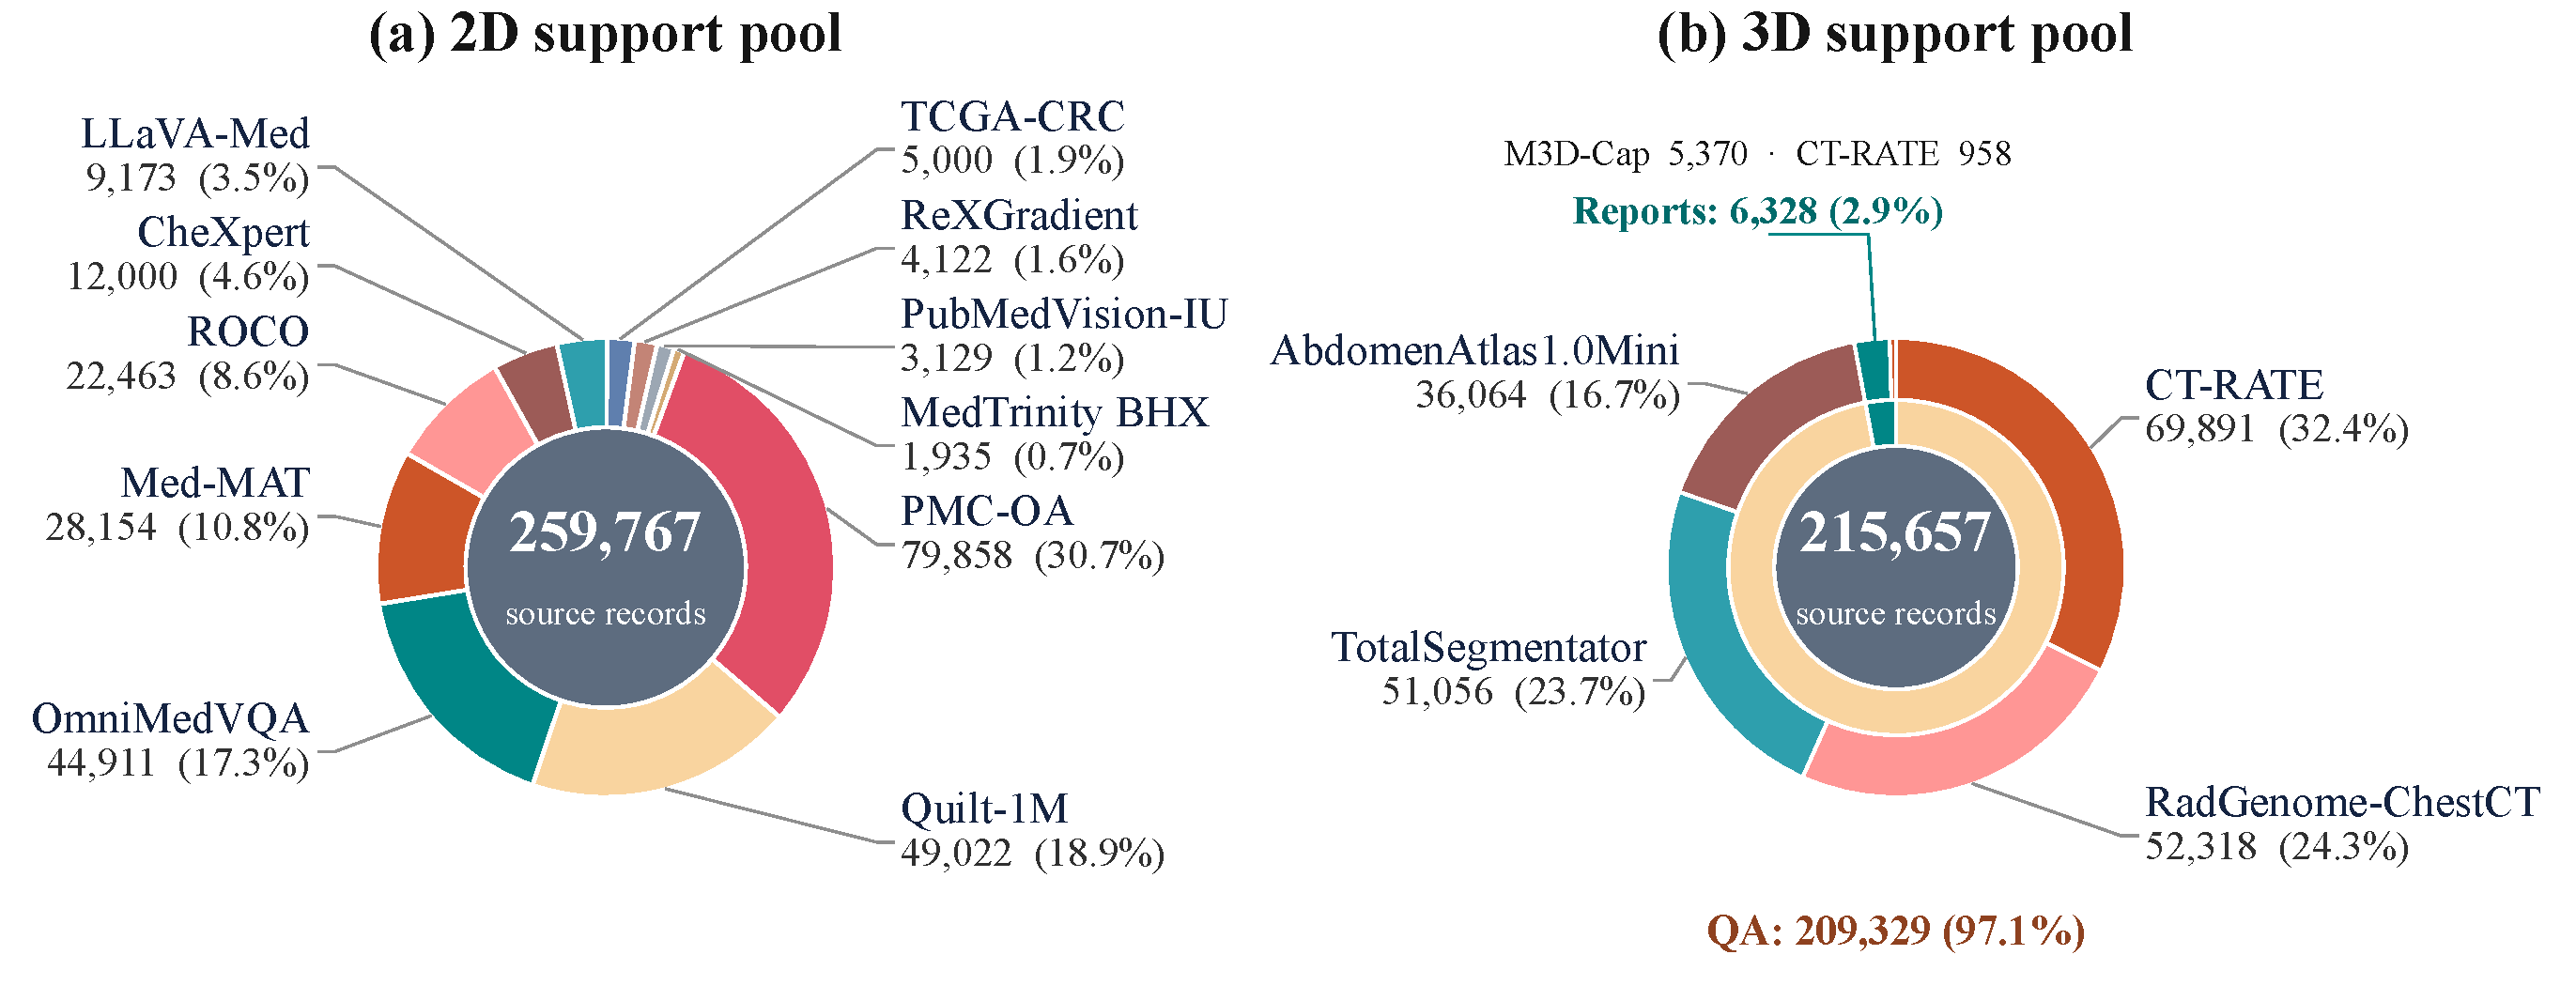
\includegraphics[width=\linewidth]{figures/support_composition.pdf}
\caption{支持集来源组成。（a）二维支持集包含259,767条源记录。（b）三维支持集包含215,657条源记录：内环区分问答与报告，外环表示相应来源。扇区面积与百分比均相对于各面板总量计算。}
\label{fig:support_composition}
\end{figure}

\begin{table}[!htbp]
\centering\small
\caption{支持集来源的官方资源。PubMedVision-IU、MedTrinity BHX 与 TCGA-CRC 的链接指向相应母数据集。}
\label{tab:support_links}
\setlength{\tabcolsep}{4pt}
\def\UrlFont{\footnotesize\sffamily}
\def\UrlBigBreaks{}
\begin{tabularx}{\linewidth}{@{}L{.28\linewidth}Y@{}}
\toprule
数据集 & 官方资源\\
\midrule
\multicolumn{2}{@{}l}{二维支持集}\\
PMC-OA\newline\citep{lin2023pmcclip} & \url{https://weixionglin.github.io/PMC-CLIP/}\\
Quilt-1M\newline\citep{ikezogwo2023quilt} & \url{https://github.com/wisdomikezogwo/quilt1m}\\
OmniMedVQA\newline\citep{hu2024omnimedvqa} & \url{https://github.com/OpenGVLab/Multi-Modality-Arena}\\
Med-MAT\newline\citep{cai2025medmat} & \url{https://github.com/FreedomIntelligence/Med-MAT}\\
ROCO\newline\citep{pelka2018roco} & \url{https://github.com/razorx89/roco-dataset}\\
CheXpert\newline\citep{irvin2019chexpert} & \url{https://aimi.stanford.edu/datasets/chexpert-chest-x-rays}\\
LLaVA-Med\newline\citep{li2023llava} & \url{https://github.com/microsoft/LLaVA-Med}\\
TCGA-CRC\newline\citep{tcga2012colorectal} & \url{https://gdc.cancer.gov/about-data/publications/coadread_2012}\\
ReXGradient\newline\citep{zhang2025rexgradient} & \url{https://huggingface.co/datasets/rajpurkarlab/ReXGradient-160K}\\
PubMedVision-IU 子集\newline\citep{chen2024pubmedvision} & \url{https://huggingface.co/datasets/FreedomIntelligence/PubMedVision}\\
MedTrinity BHX\newline\citep{xie2025medtrinity} & \url{https://github.com/UCSC-VLAA/MedTrinity-25M}\\
\midrule
\multicolumn{2}{@{}l}{三维支持集}\\
AbdomenAtlas1.0Mini\newline\citep{li2024abdomenatlas} & \url{https://huggingface.co/datasets/AbdomenAtlas/AbdomenAtlas1.0Mini}\\
CT-RATE\newline\citep{hamamci2026ctrate} & \url{https://huggingface.co/datasets/ibrahimhamamci/CT-RATE}\\
RadGenome-ChestCT\newline\citep{zhang2025radgenome} & \url{https://huggingface.co/datasets/RadGenome/RadGenome-ChestCT}\\
TotalSegmentator\newline\citep{wasserthal2023totalsegmentator} & \url{https://github.com/wasserth/TotalSegmentator}\\
M3D-Cap\newline\citep{bai2024m3d} & \url{https://huggingface.co/datasets/GoodBaiBai88/M3D-Cap}\\
\bottomrule
\end{tabularx}
\end{table}
